\section{Experimental Evaluation: Deterministic Forecasting}
\label{sec:deterministic}

In this section, we present the results on deterministic out-of-sample forecast. We are interested in particularly the following questions:
(1) Do neural residual models outperform  purely nonlinear neural models and purely physical model? (2) Does more synthetic data from climate model simulations benefit the prediction performance?

\subsection{Experimental Setup}
\paragraph{Climate Indices and Dataset:} The ENSO indices include sea surface temperature anomalies averaged over Ni\~no 3.4 region 170$^\circ$-120$^\circ$W, 5$^\circ S$-5$^\circ$N (T) and the depth of the 20 $^\circ C$ subsurface isotherm averaged over the equatorial Pacific 120$^\circ$E-80$^\circ$W, 5$^\circ S$-5$^\circ$N (h). The non-ENSO climate-modes climate modes in other ocean basins (i.e., $\bX_M^\top$) are defined based on area-weighted means of sea surface temperature anomalies: three in the Indian Ocean, two in the Pacific (North/South), and three in the Atlantic (North/South/equatorial) (Appendix B). For observational dataset, we utilize the SST and three-dimensional subsurface ocean temperature produced by ECMWF Ocean Reanalysis System 5 (ORAS5), ranging from 1958-2023 \cite{zuo2019oras5}. The training period spans January 1979 through December 2001, comprising 276 monthly observations over 23 years. The test period spans January 2002 through December 2022, comprising 252 monthly observations over 21 years. We evaluate ENSO forecasts at lead times from 1 to 21 months, covering the operationally-relevant horizon for ENSO prediction. In the transfer-learning experiment, we use $100$ members of large ensemble historical simulations from Community Earth System Model, version 2 (CESM) \cite{LENS}. For each CESM ensemble member, we extract the same set of climate indices and temporal ranges as in the observation data.

\paragraph{Evaluation Metrics:} We use root mean squared error (RMSE) to measure the typical magnitude of forecast errors in degrees Celsius, with lower values indicating better performance, and anomaly correlation coefficient (ACC), which measures the linear association between forecasts and observations. These two metrics are standard for evaluating deterministic ENSO forecast \cite{zhao2024xro, TangangTangMonahanHsieh1998NNEOF, KondrashovKravtsovRobertsonGhil2005EMR}. 

\paragraph{Baselines:}To better understand the first question above, we include models that are purely neural (fully-nonlinear Neural ODE \cite{chen2018neuralode}, transformer \cite{vaswani2017attention}), purely physical (XRO \cite{zhao2024xro}), and a large number of neural residual models, including NXRO-MLP, NXRO-Graph, NXRO-Attentive, and $35$ others, covering extensive neural architectural search (full list in Appendix \ref{app:a1}). The baseline Neural ODE model takes the generic form as in ~\cite{chen2018neuralode}, which parametrizes the entire vector field  as a 3-layer MLP. As for the transformer model, we use the tokenization approach from models like Informer  \cite{zhou2021informerefficienttransformerlong} and Autoformer \cite{wu2022autoformerdecompositiontransformersautocorrelation}, which tokenizes the time series variables alongside the time stamps, encoding month-of-year and providing  periodic information. These models vary significantly on their parameter counts, with NXRO-GCN and NXRO-Attention model taking $\sim 260$ times fewer parameters than the transformer baseline. We provide  hyperparameter details in Appendix \ref{app:a1}.  


\subsection{Training Strategy and Data Source}
 
To study the second question, we examine whether pre-training on related datasets can improve generalization~\cite{pan2010transfer,weiss2016survey, pmlr-v202-nguyen23a, bodnar2025earthsystemfm} and investigate a two-stage training procedure: In the first stage, we train the model on synthetic climate indices derived from CESM  climate model simulations. The goal is to learn general features of climate variability that transfer to the real system. In the second stage, we fine-tune the pre-trained model on the observational data \cite{zuo2019oras5}. The pre-trained weights provide an initialization that may be closer to good solutions than random initialization, potentially enabling faster convergence and better generalization. 

\subsection{Overall Performance Comparison}

% \begin{table}[t]
\centering
\label{tab:rmse_selected_leads}
\setlength{\tabcolsep}{3.5pt} % tighten column spacing
\renewcommand{\arraystretch}{1.15}
\begin{tabular}{rcccccc}
\toprule
Lead & XRO & \shortstack{NXRO\\Attn} & \shortstack{NXRO\\GNN} & \shortstack{NXRO\\MLP} & \shortstack{Neural\\ODE} & \shortstack{Trans\\former} \\
\midrule
3  & 0.350 & 0.289 & 0.298 & \textbf{0.275} & 0.401 & 0.406 \\
6  & 0.558 & 0.456 & 0.479 & \textbf{0.440} & 0.628 & 0.622 \\
9  & 0.659 & 0.571 & 0.598 & \textbf{0.571} & 0.718 & 0.749 \\
12 & 0.704 & \textbf{0.659} & 0.682 & 0.672 & 0.786 & 0.858 \\
15 & 0.763 & \textbf{0.740} & 0.750 & 0.778 & 0.859 & 0.948 \\
18 & 0.809 & 0.787 & \textbf{0.785} & 0.851 & 0.872 & 0.987 \\
21 & 0.833 & 0.807 & \textbf{0.801} & 0.883 & 0.856 & 0.968 \\
\midrule
Parameters & 650 & 633 & 537 & 6334 & 5514 & $\sim$ 170K \\ 
\bottomrule
\end{tabular}
\caption{RMSE at selected lead times  for the models explored in Figure \ref{fig:1c_core_models_ranking}. Best (lowest) RMSE per row is in bold. We see a clear pattern that MLP based nonlinear component performs the best at short-term, while attention starts to pick up at medium-term, and GNN at long-term. Overall all the NXRO variants consistently outperform the XRO baseline and the purely non-physical models.}
\end{table}

\begin{figure}
    \centering
    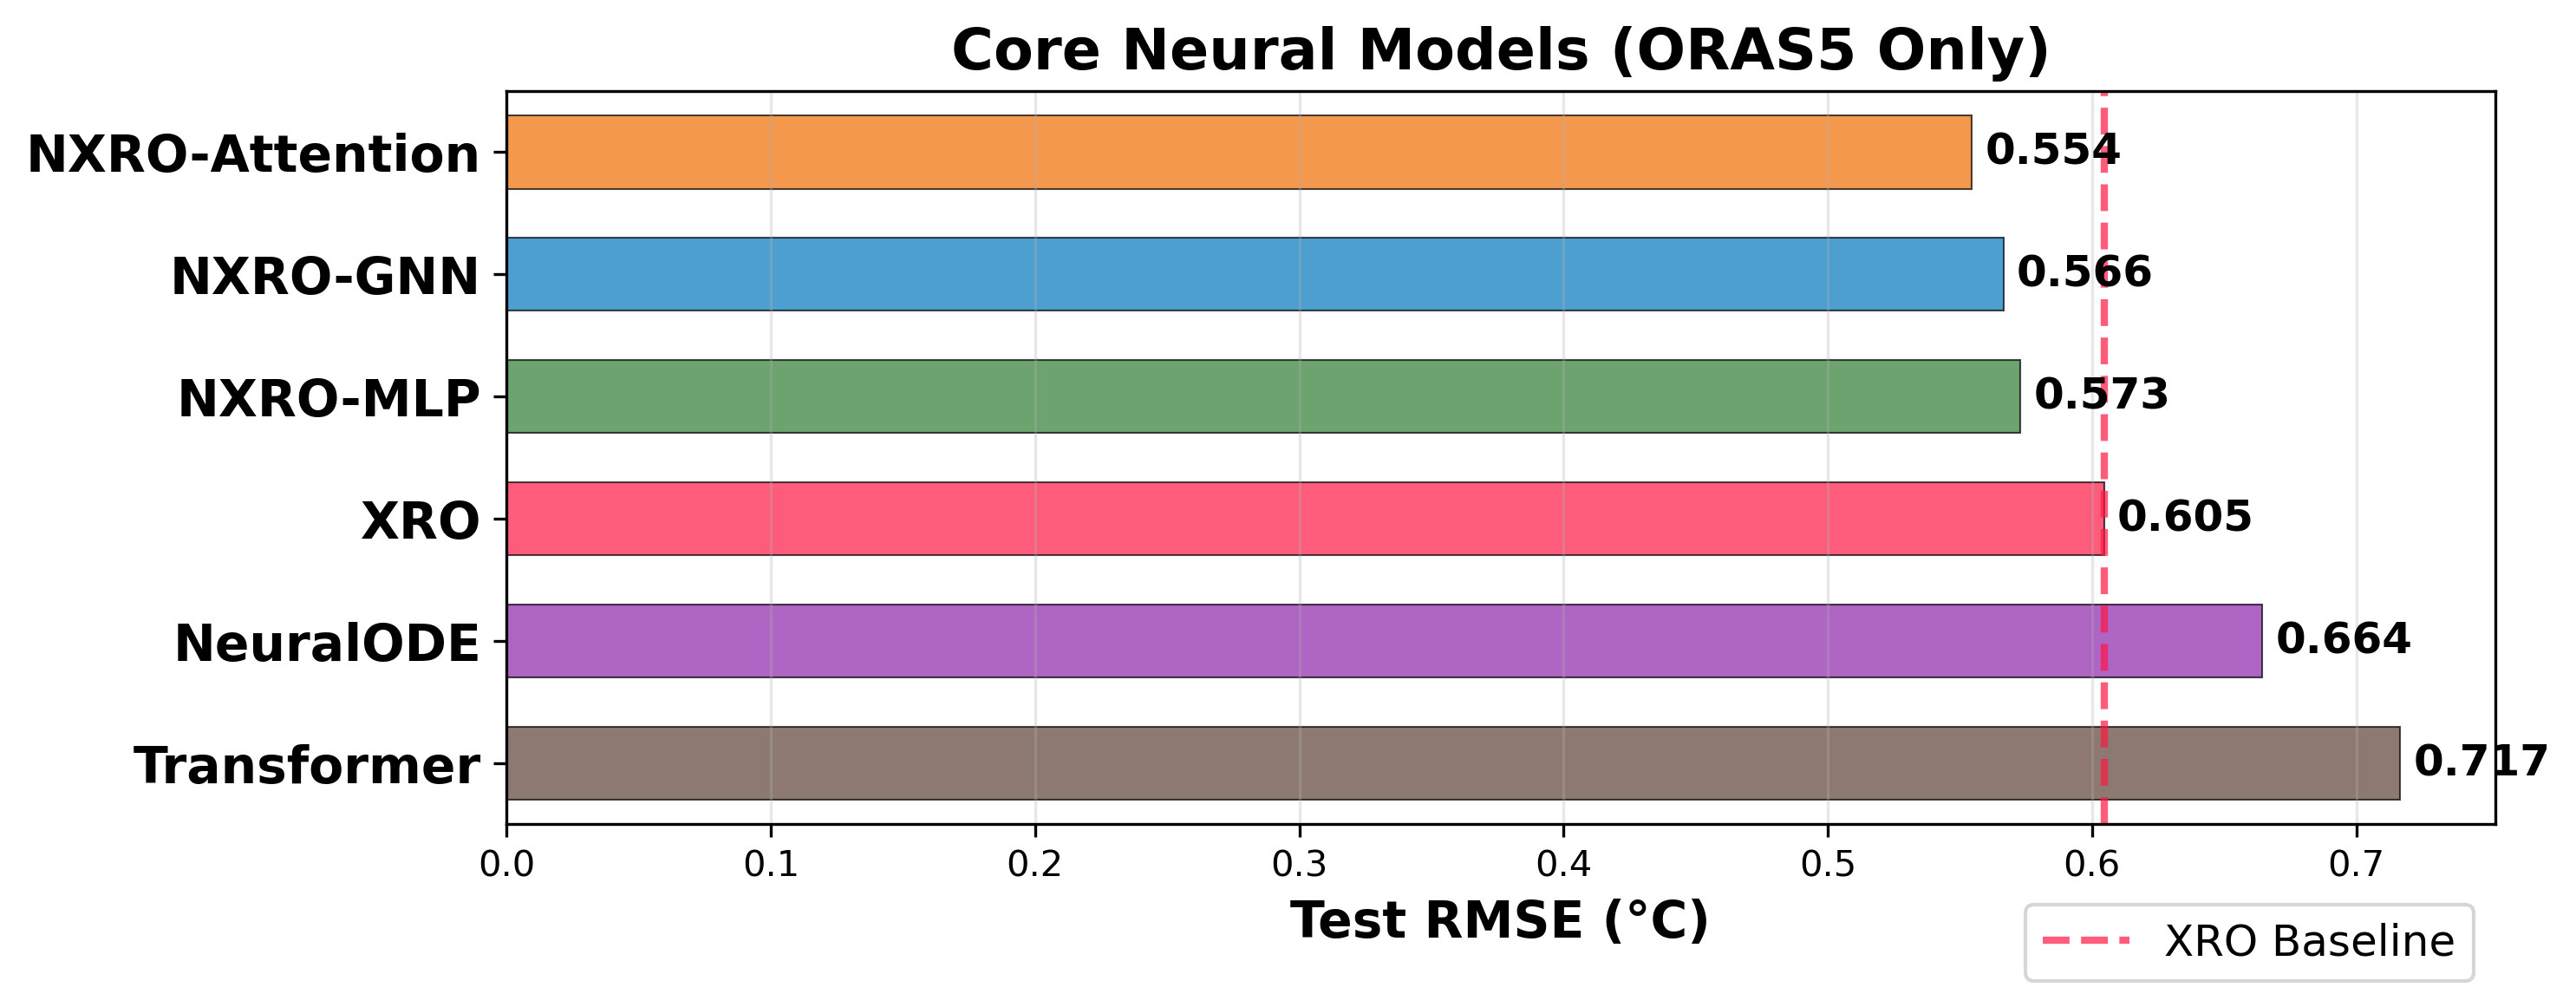
\includegraphics[width=\columnwidth]{figures/1c_core_models_ranking.png}
    \caption{Average RMSE across 21 lead times on the out-of-distribution ENSO forecast. NXRO variants outperform baselines by a significant margin.}
    \label{fig:1c_core_models_ranking}
\end{figure}
\begin{table}[t]
\centering
\setlength{\tabcolsep}{3.5pt} % tighten column spacing
\renewcommand{\arraystretch}{1.15}
\begin{tabular}{rccc@{\hspace{6pt}\vrule\hspace{6pt}}cccc}
\toprule
Lead & \shortstack{Neural\\ODE} & \shortstack{Trans\\former} & XRO & \shortstack{NXRO-\\MLP} & \shortstack{NXRO-\\Attn} & \shortstack{NXRO-\\GNN} \\
\midrule
3  & 0.401 & 0.406 & 0.350 & \textbf{0.275} & 0.289 & 0.298 \\
6  & 0.628 & 0.622 & 0.558 & \textbf{0.440} & 0.456 & 0.479 \\
9  & 0.718 & 0.749 & 0.659 & \textbf{0.571} & 0.571 & 0.598 \\
12 & 0.786 & 0.858 & 0.704 & 0.672 & \textbf{0.659} & 0.682 \\
15 & 0.859 & 0.948 & 0.763 & 0.778 & \textbf{0.740} & 0.750 \\
18 & 0.872 & 0.987 & 0.809 & 0.851 & 0.787 & \textbf{0.785} \\
21 & 0.856 & 0.968 & 0.833 & 0.883 & 0.807 & \textbf{0.801} \\
\midrule
Parameters & 5514 & $\sim$ 170K & 650 & 6334 & 633 & 537 \\
\bottomrule
\end{tabular}
\caption{RMSE at selected lead times  for the models explored in Figure \ref{fig:1c_core_models_ranking}. Best (lowest) RMSE per row is in bold. We see a clear pattern that MLP based nonlinear component performs the best at short-term, while attention starts to pick up at middle-term, and GNN at long-term.}
\label{tab:rmse_selected}
\end{table}

\begin{figure}
    \centering
    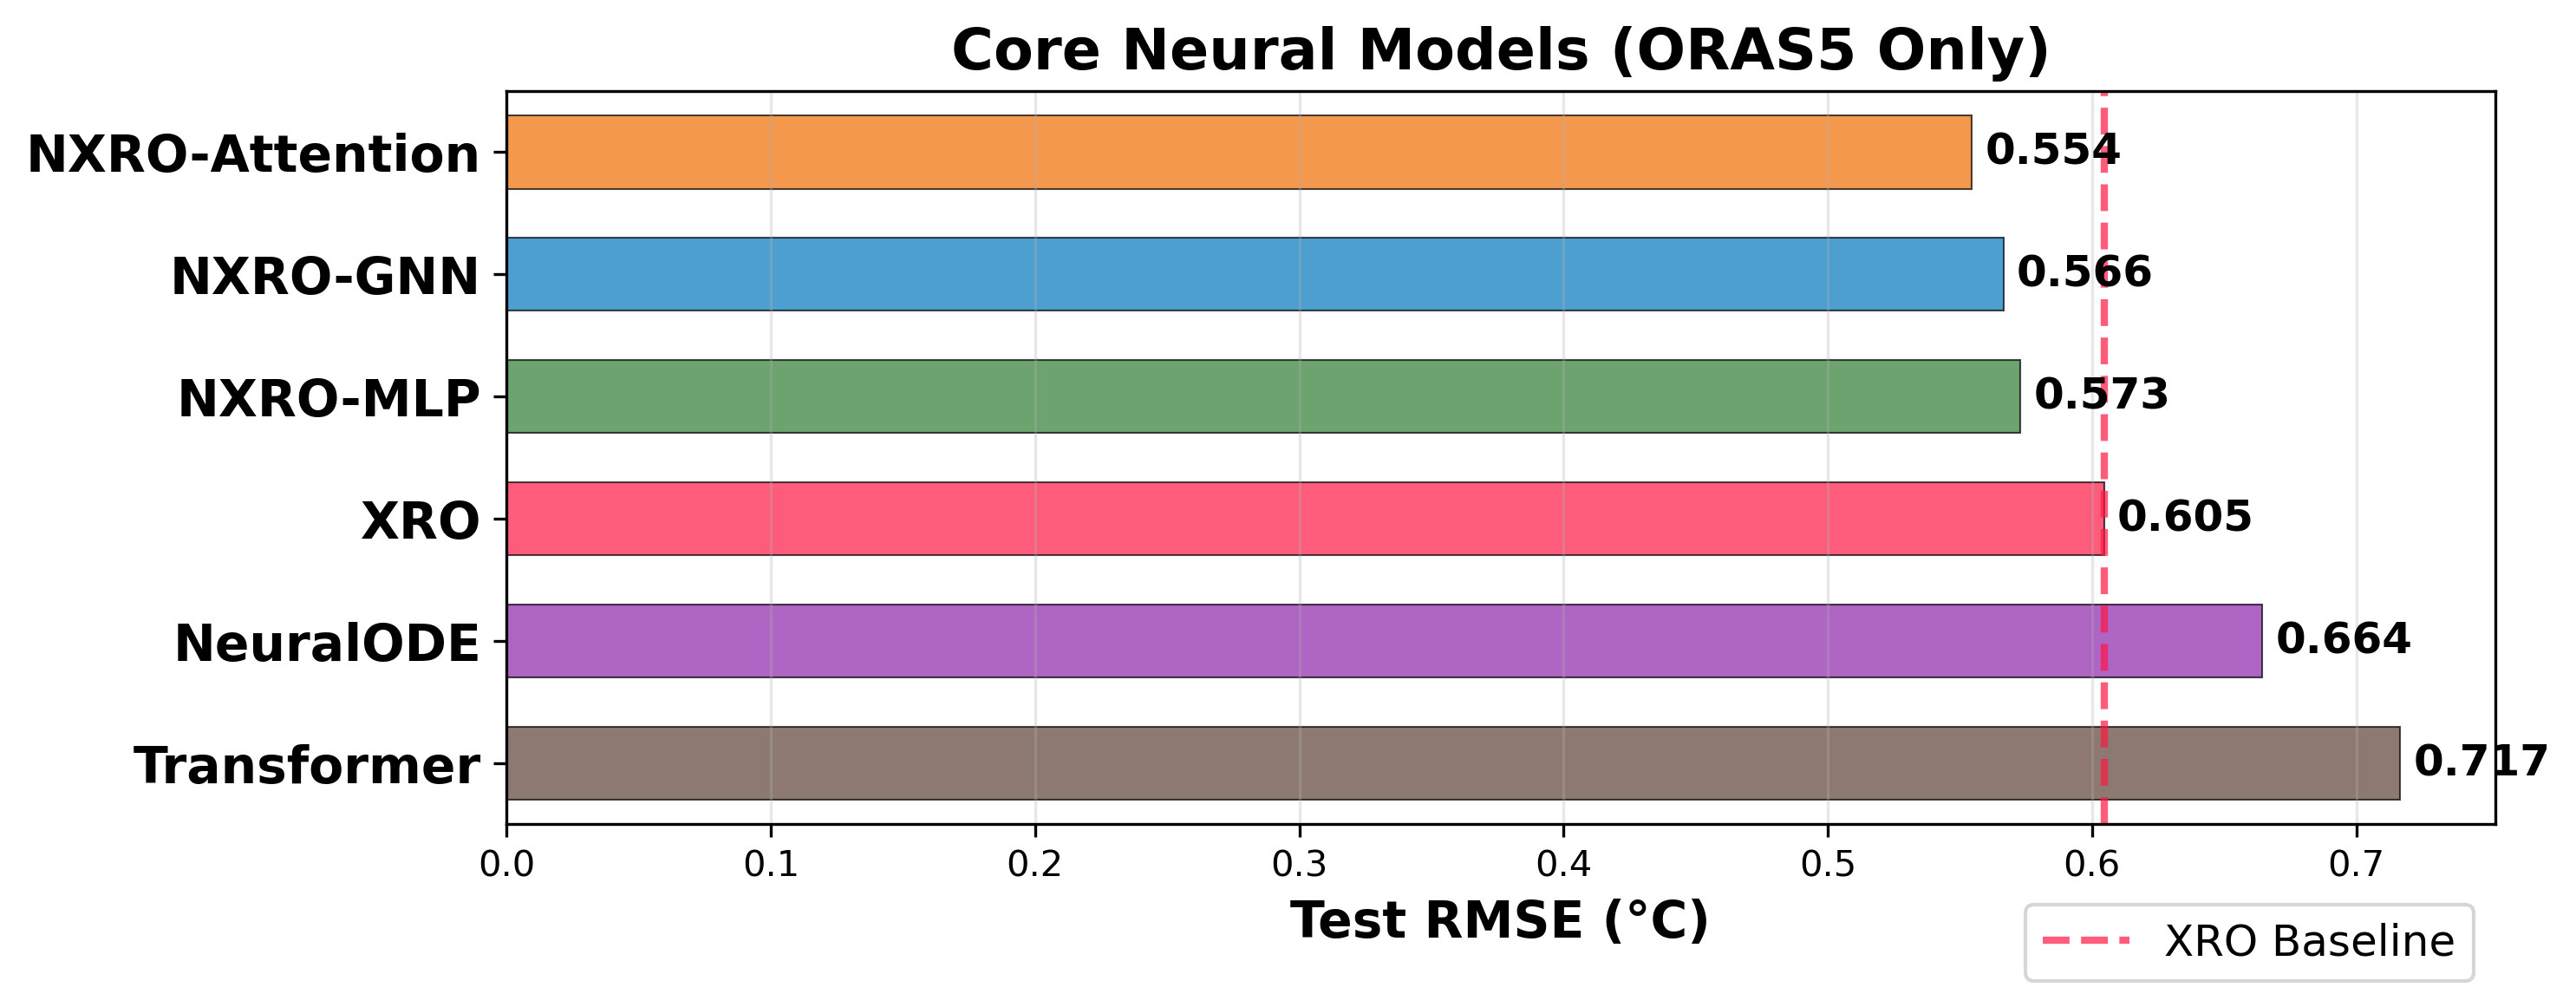
\includegraphics[width=\columnwidth]{figures/1c_core_models_ranking.png}
    \caption{Average RMSE across 21 lead times on the out-of-distribution ENSO forecast. NXRO variants outperform baselines by a significant margin.}
    \label{fig:1c_core_models_ranking}
\end{figure}

Figure \ref{fig:1c_core_models_ranking} presents the average predictive performance of the NXRO-variants, the physical XRO model, a fully nonlinear Neural ODE model, and a transformer model. The attention based neural model (NXRO-Attention) achieves the best average out-of-sample performance, with an average test RMSE of 0.554°C. This represents a 8.4\% improvement in RMSE to the XRO baseline. All variants of nonlinearity presented in Section 3 outperform the XRO baseline. Notably, the purely neural transformer model overfits severely to the small dataset, resulting in poor prediction performance. For more granular comparisons at the temporal scale, we also provide in Table \ref{tab:rmse_selected} the test RMSE at lead times $3,6,\cdots 21$ months, where a clear pattern emerges that the NXRO-MLP model variant outperforms at short lead time, but NXRO-Attention excels at medium lead time, and ultimately NXRO-GNN model dominiates at longer lead times.


Figure~\ref{fig:top10_rmse} shows the most granular comparison between the models by displaying RMSE as a function of forecast lead time for the top models: notably, the Graph based residual model  performs consistently better than the XRO model at all lead times, and the pattern from Table \ref{tab:rmse_selected} persists.  These results demonstrate that the neural ODE based residual models (NXRO variants) outperform the base XRO model in different ways and validate their effectiveness for ENSO forecast, highlighting the importance of a neural correction term. Moreover, the poor performance of the fully nonlinear neural ODE and the transformer model signals the importance of the linear component and its associated physical prior. We provide comprehensive results for all the model variants we have experimented on in Appendix A. 

\begin{figure*}[htbp]
    \centering
    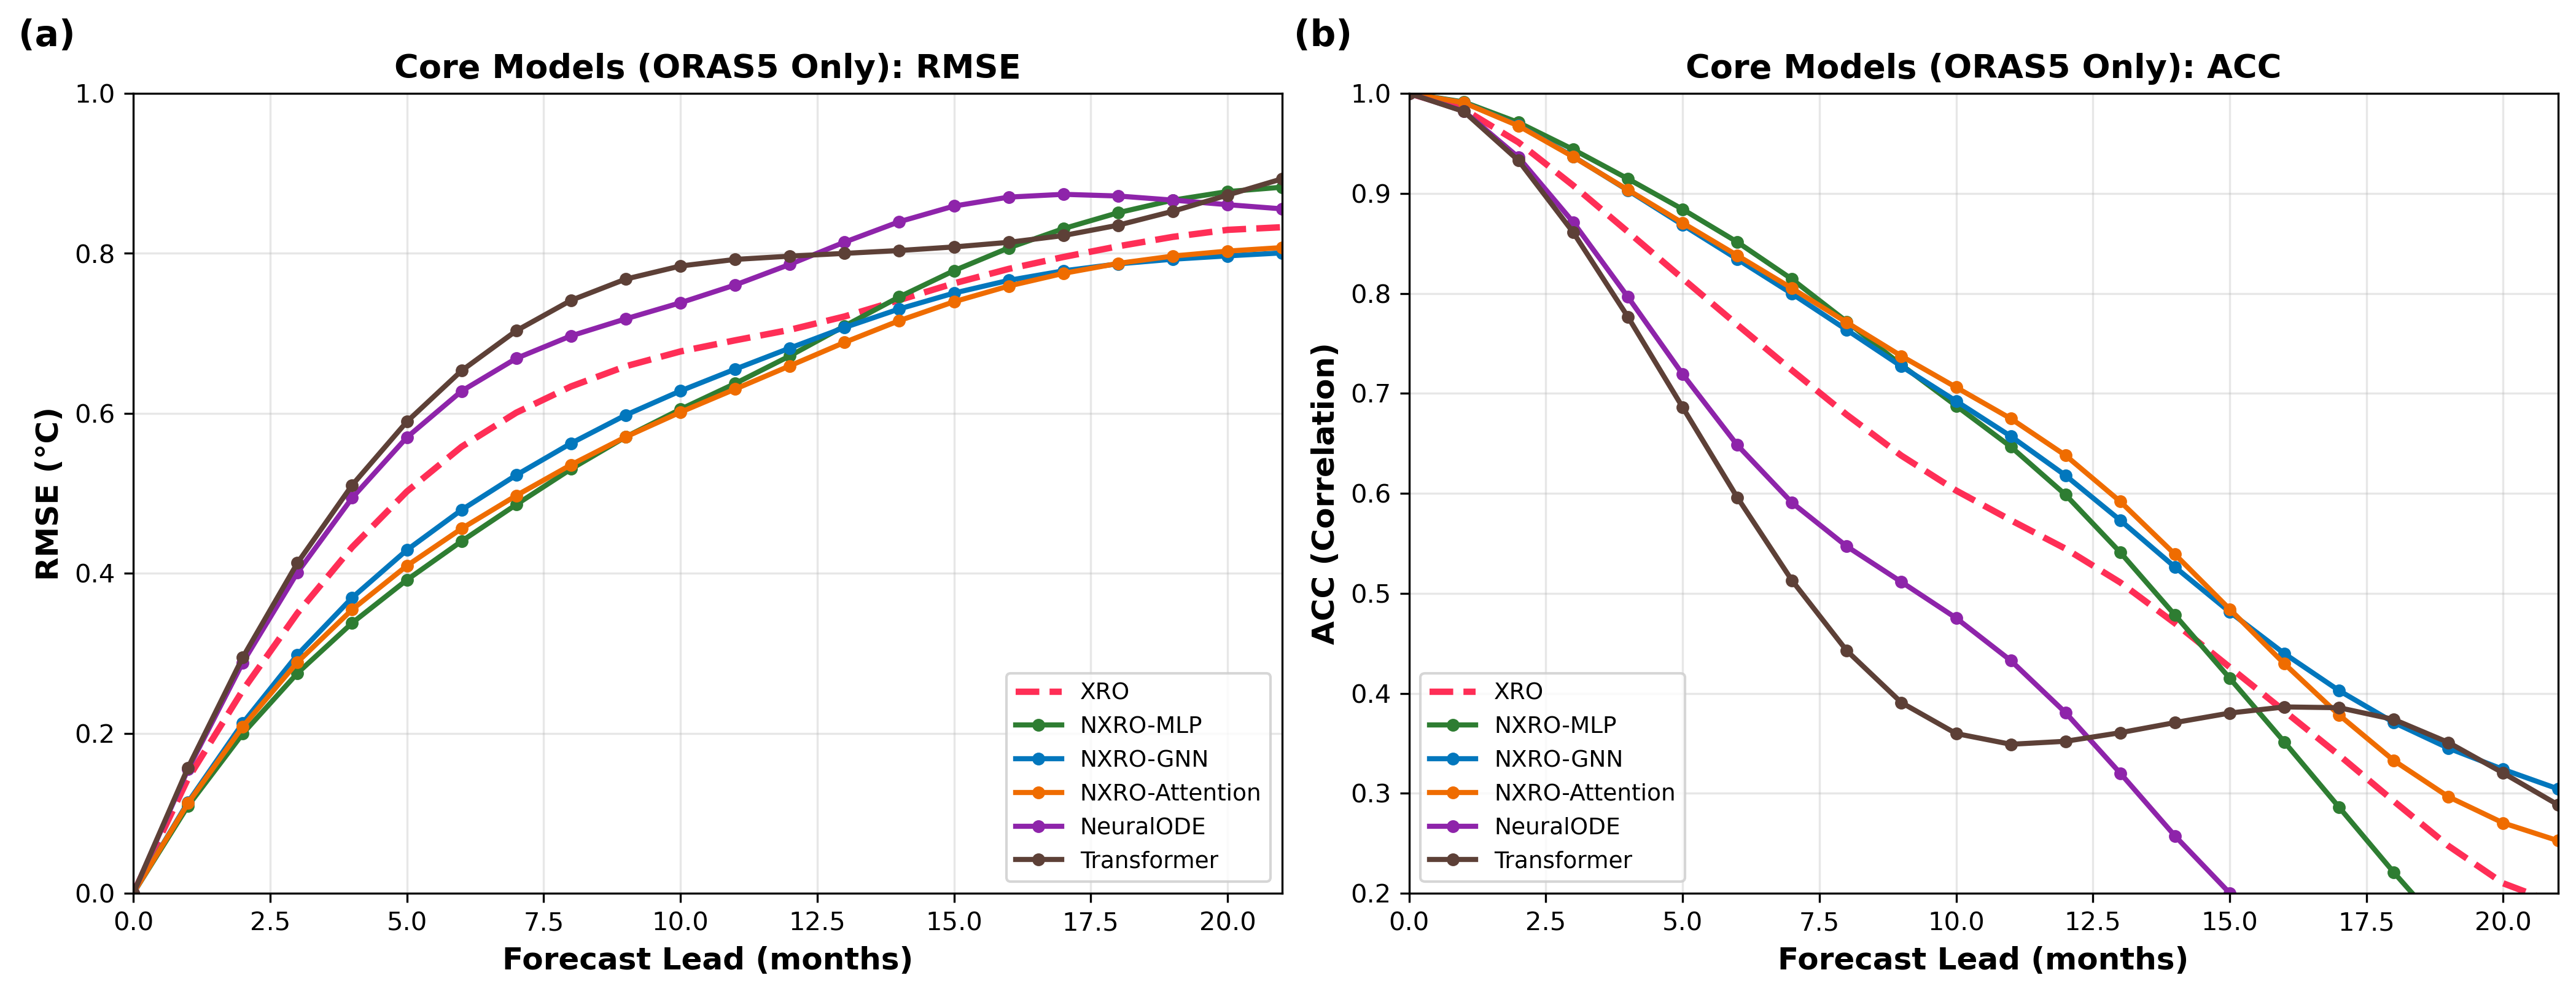
\includegraphics[width=\textwidth]{figures/1f_core_models_combined.png}
    \caption{Out-of-sample results for (a) RMSE and (b) Anomaly Correlation Coefficient (ACC) as a function of forecast lead time. The residual model achieves lowest error at all leads (MLP for short and medium, graph and attention modules at all lead times) than the baseline XRO model.}
    \label{fig:top10_rmse}
\end{figure*}


\subsection{Transfer Learning Analysis}

We investigate whether pre-training on synthetic climate data can improve generalization~\cite{pan2010transfer}. The two-stage training procedure first trains on CESM-derived climate indices using the same year range, then fine-tunes on the observational data. Figure~\ref{fig:two_stage_a} compares observations only and pretraining+fintuning results across model variants. For the NXRO-variants explored in Table \ref{tab:rmse_selected}, we can observe that the effect of pre-training actually degrades the test performance, although the performance varies dramatically across  architectures (shown in Appendix A).  This counterintuitive result arises because the synthetic climate data, while realistic, contains systematic biases relative to observations. The MLP learns to correct for these biases during pre-training, but these corrections are inappropriate for the real system. This asymmetry suggests a principle for transfer learning in hybrid models: pre-training benefits components that encode general structure. When the pre-training distribution differs from the target distribution, flexible components may learn spurious patterns that are difficult to unlearn. This observation may suggest that modeling physical systems should adhere to two paradigms: either a data-centric method that relies on massive scales of climate simulation datasets (such as foundation models) or physics-based hybrid model based on real observational data. Our study suggests that the approach that aims in-between these two paradigm usually results in worse predictive performance for the task of ENSO forecast.


\begin{figure}[t]
  \centering
    \centering
    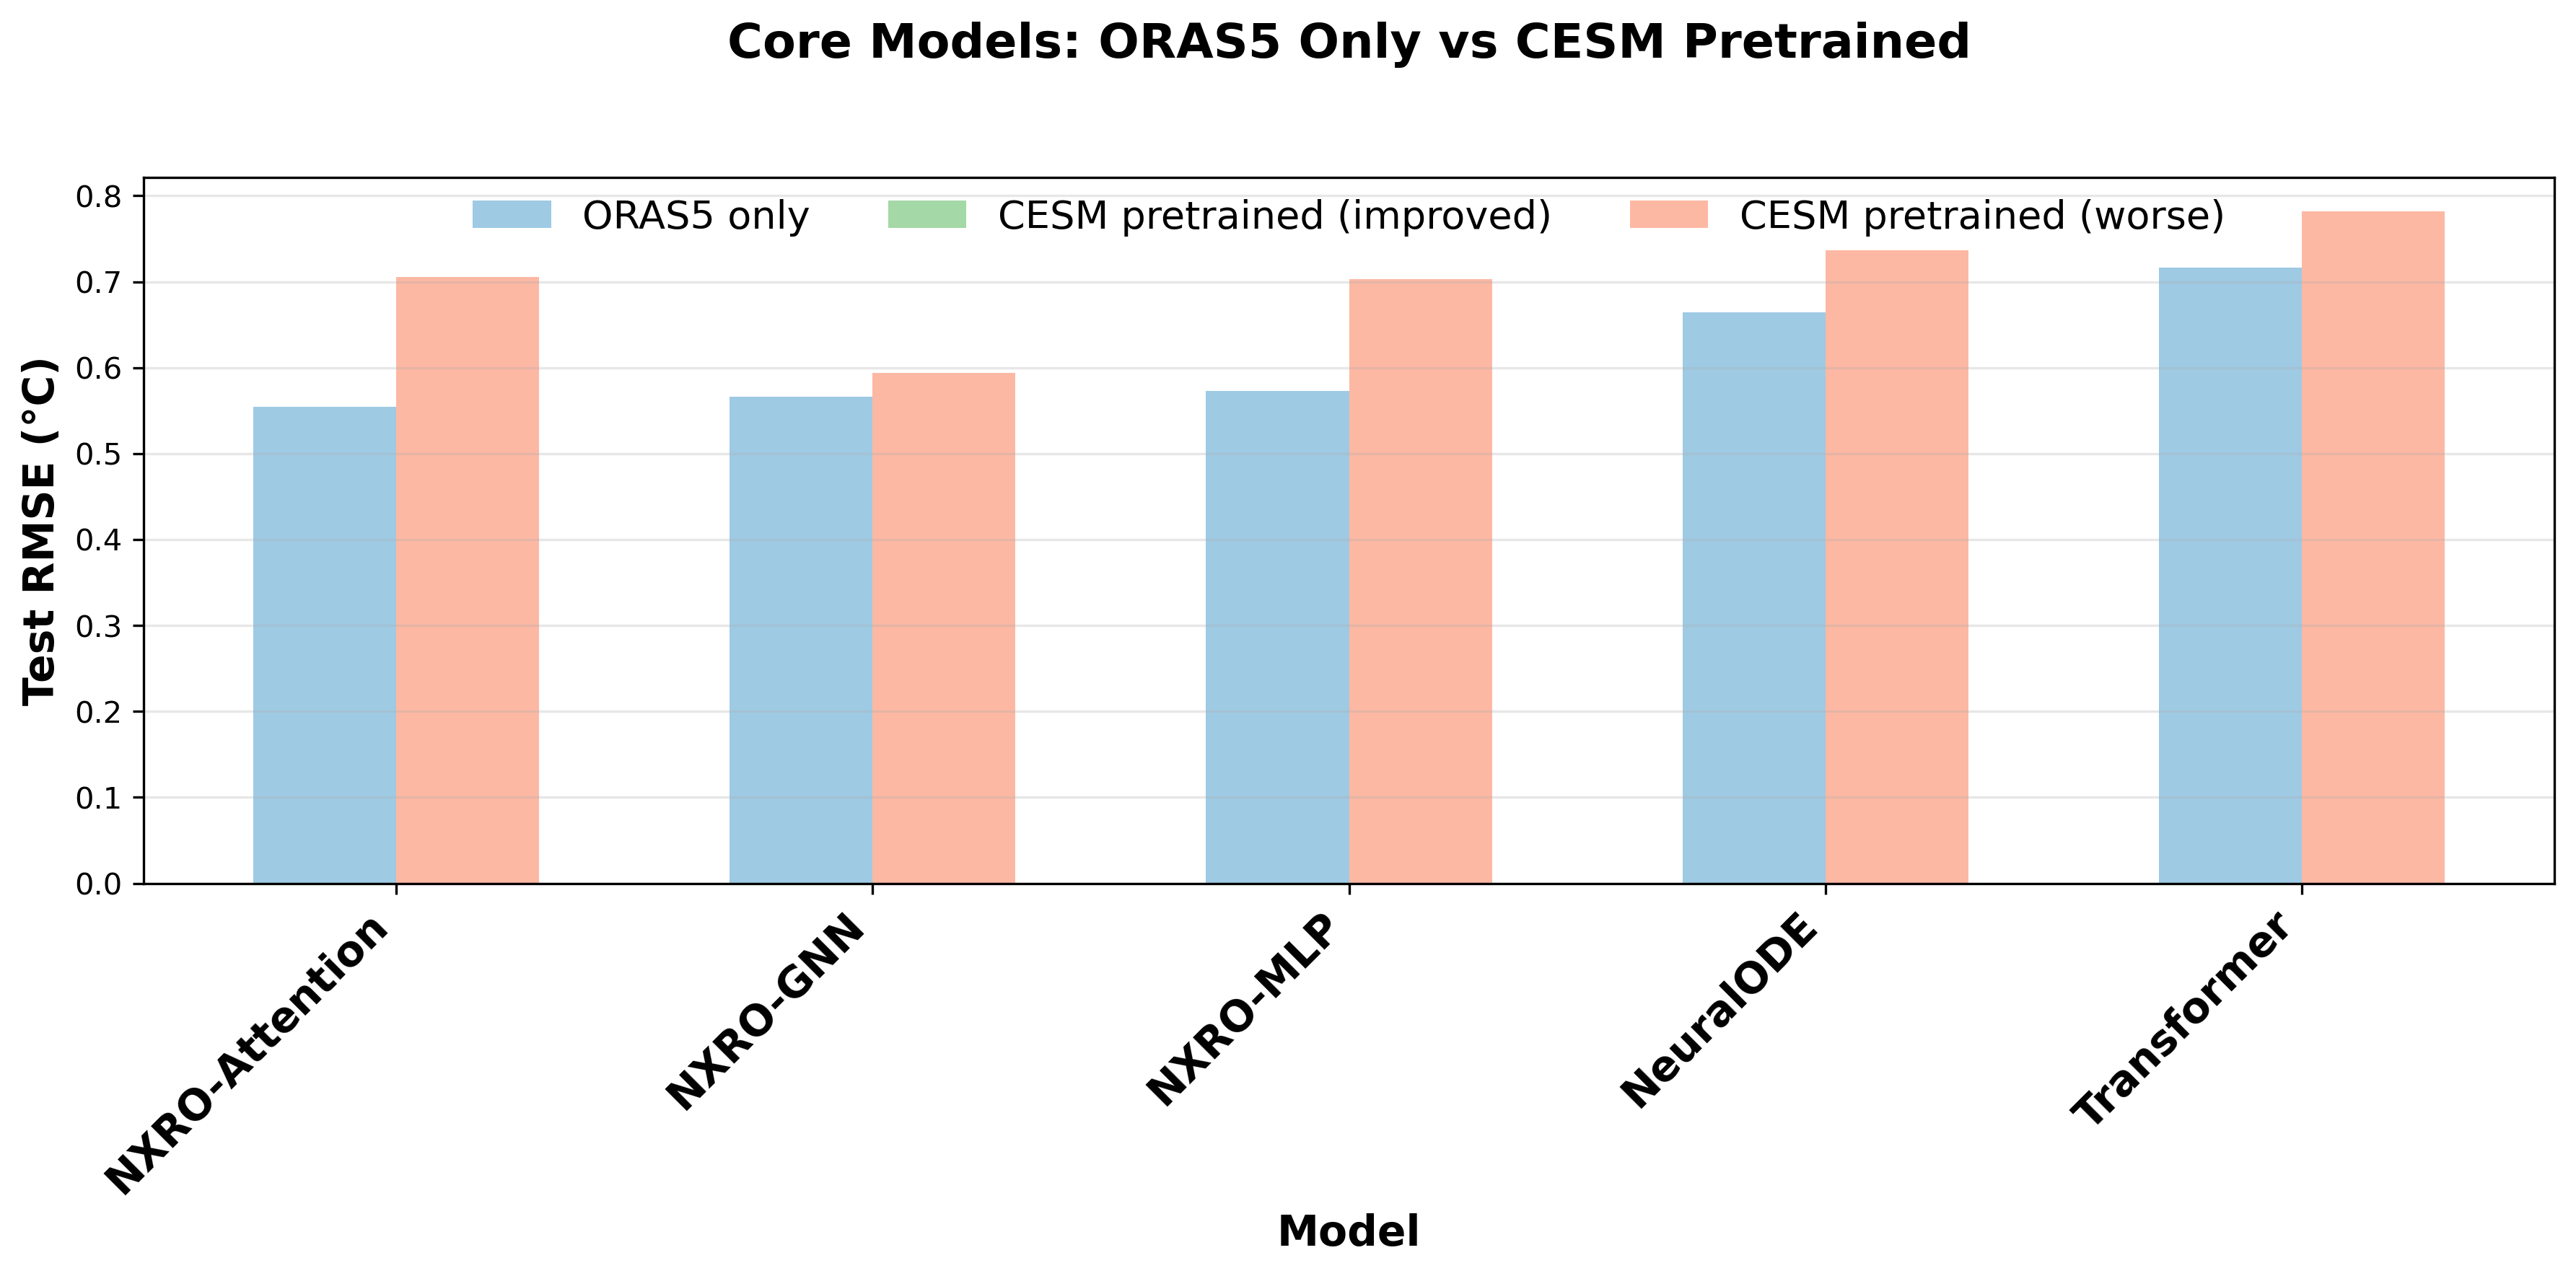
\includegraphics[width=\linewidth]{figures/6d_core_models_single_vs_two_stage.png}
    \caption{Average Test RMSE for ENSO forecast. Comparison of ORAS5 training only vs.\ pretraining on CESM and finetuning on ORAS5. Green bars indicate better performance with CESM; red bars indicate worse.}
    \label{fig:two_stage_a}
\end{figure}




\subsection{Teleconnection Through Graph Structure Learning}

On top of the consistently better performance than the baseline XRO model and the fully nonlinear neural models, our XRO-GNN model defined in equation \ref{eq:nxro_graph} provides the additional benefit of \textit{explainability-by-design}. The mathematical formulation of NXRO-GNN in equation \ref{eq:nxro_graph} includes both the learned linear coupling term $L_\theta(t)$, the nonlinear interaction residual term $\text{GNN}_{\theta}$, and the seasonal gating term $\alpha(t)$. Moreover, the graph structure, encoded by an adjacency matrix, is set to be learnable. By studying these learned components after training, we can hope to uncover the mechanisms discovered by the model that exhibits robust predictive performance. 
    
\begin{figure}[t]
    \centering
    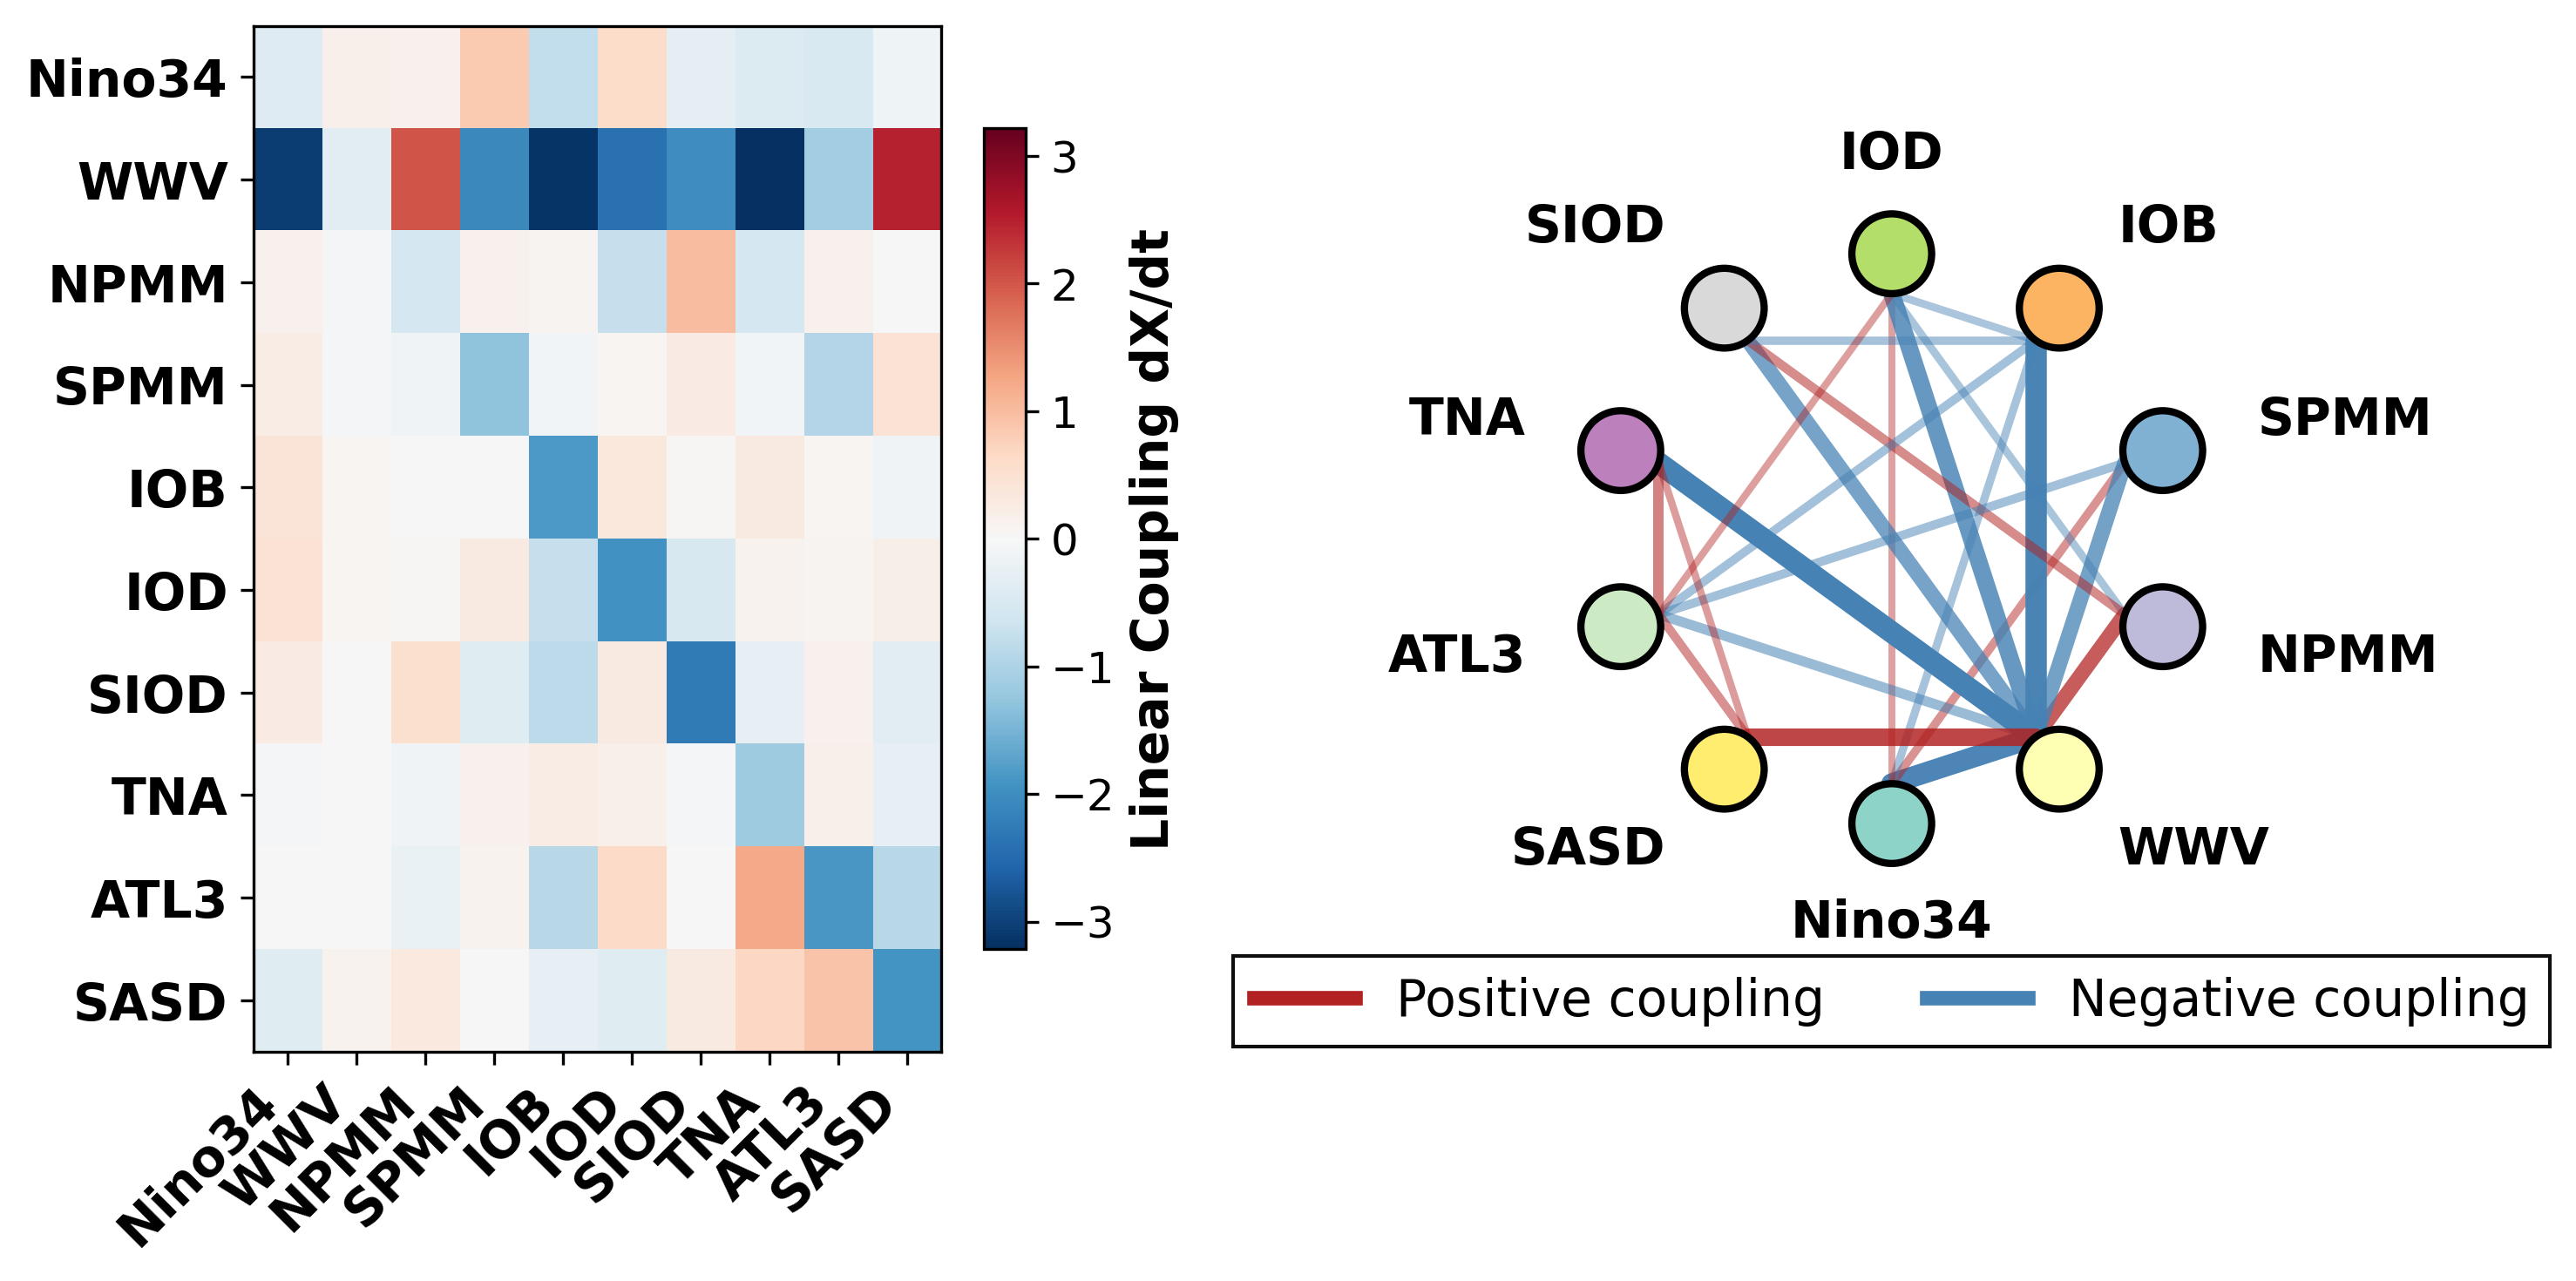
\includegraphics[width=\linewidth]{figures/linear_coupling_L.png}
    \caption{The linear coupling strength between all the climate modes extracted from the learned NXRO-GNN model. Thicker lines and darker color indicates stronger interaction.}
    \label{fig:gnn_linear_coupling}
\end{figure}

\begin{figure}[t]
  \centering
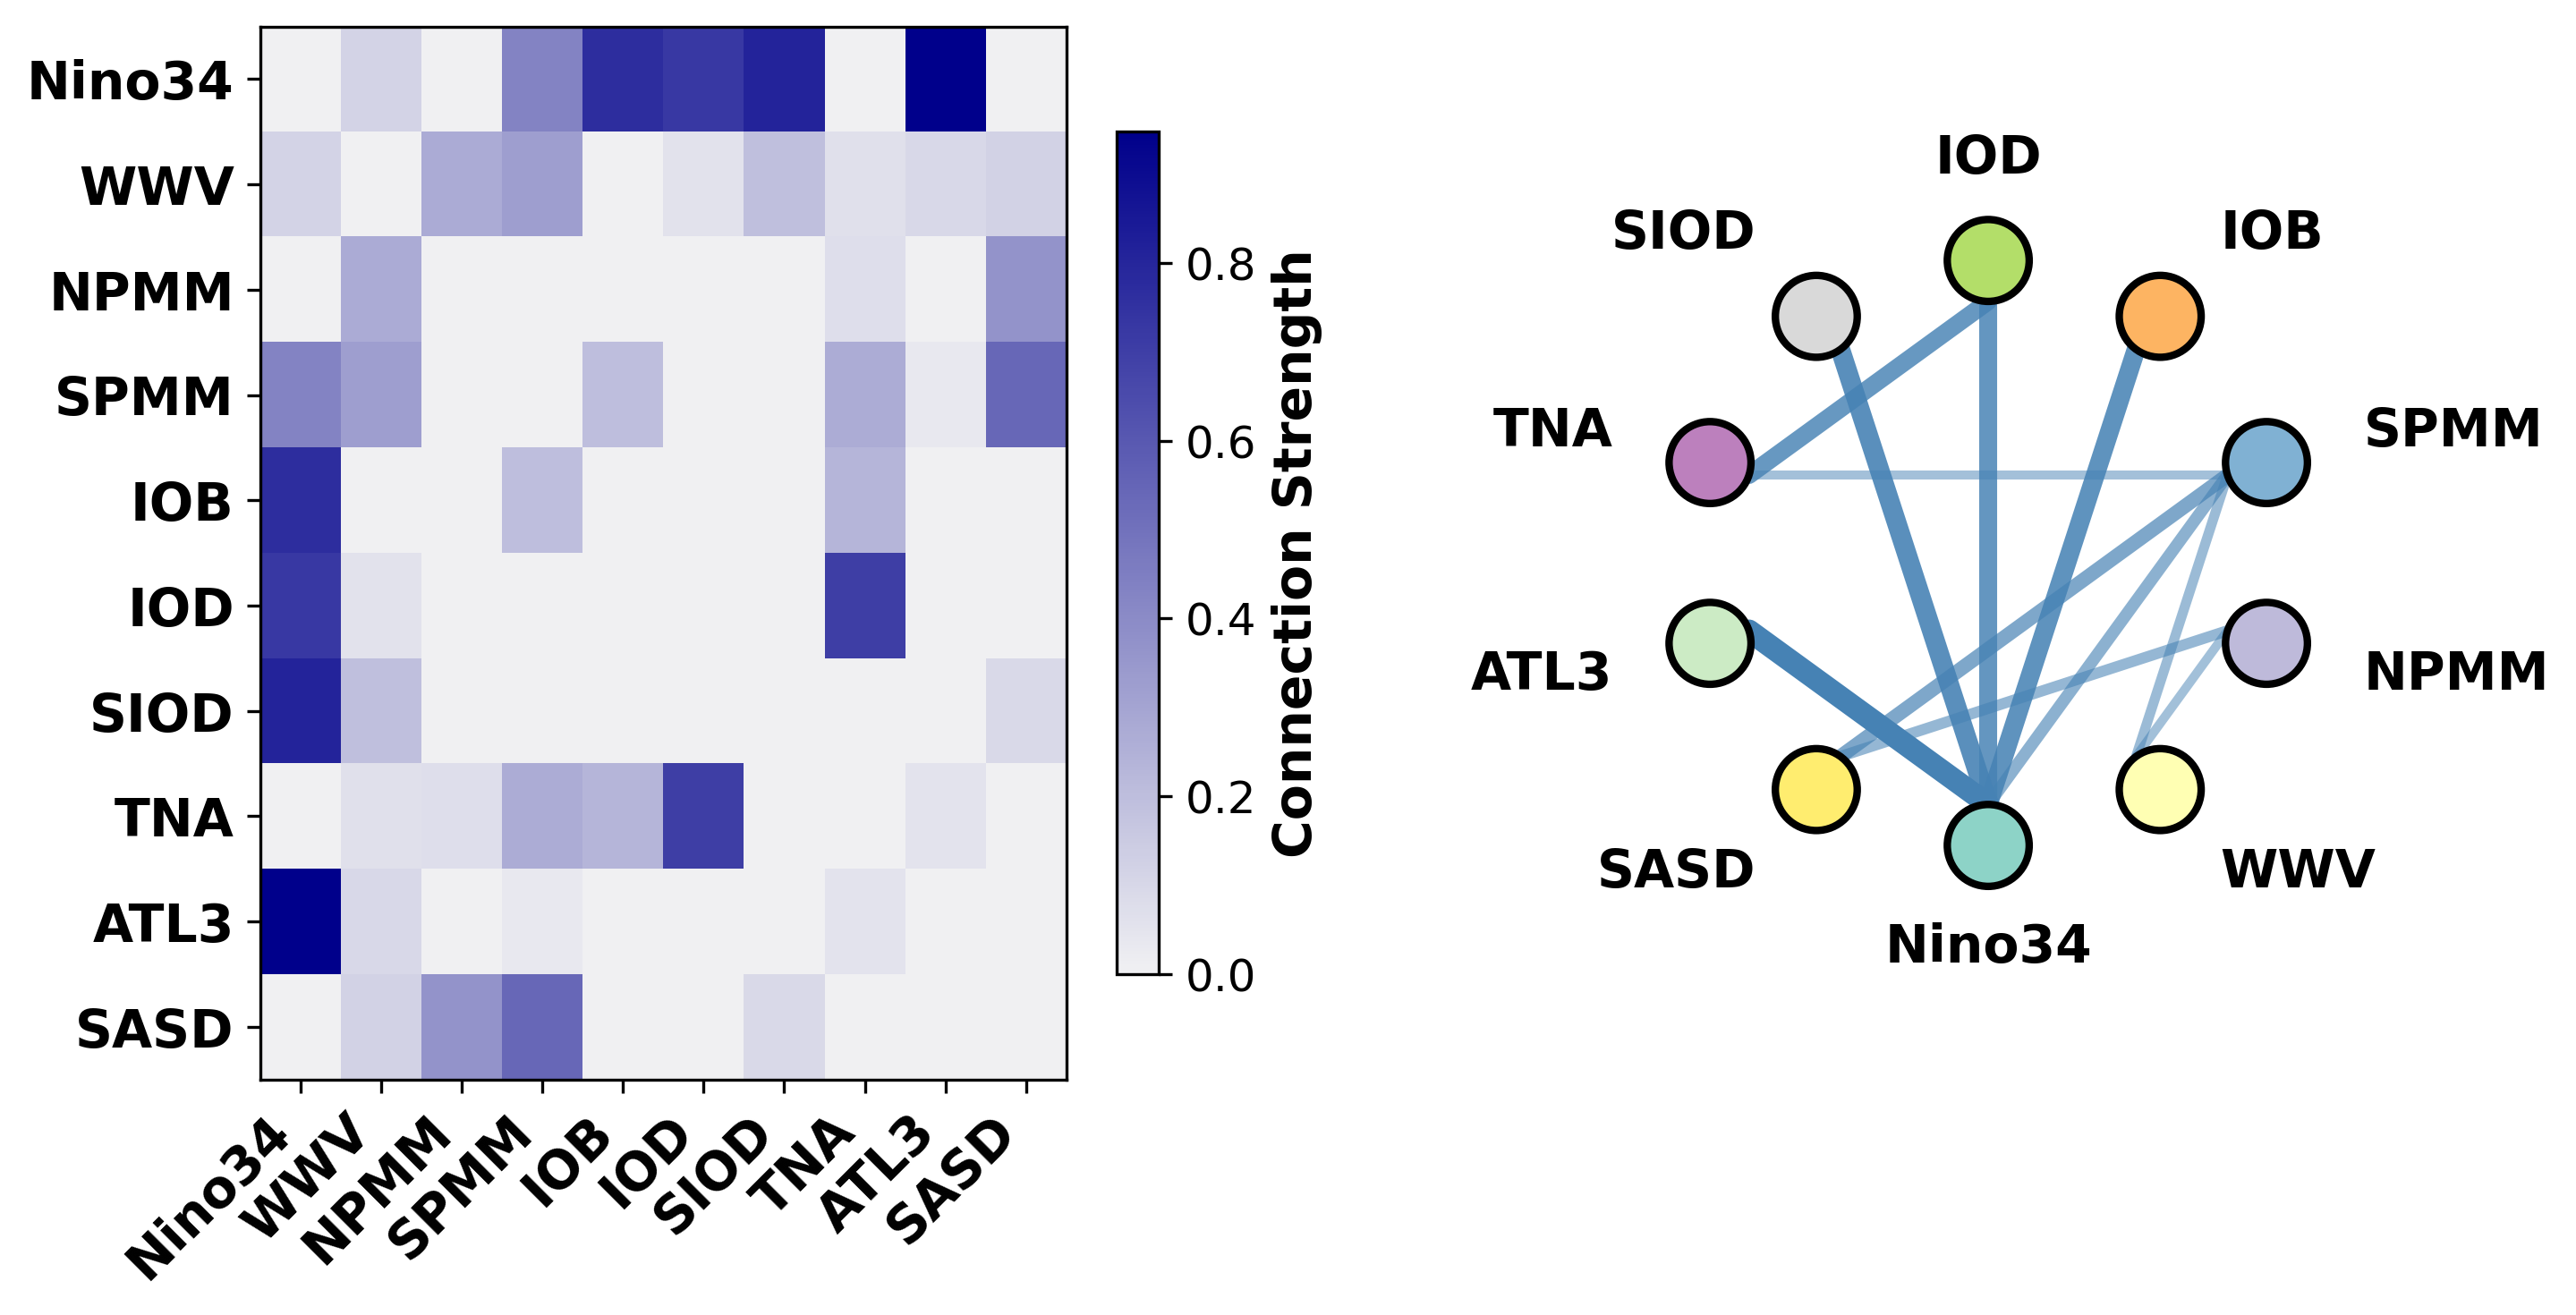
\includegraphics[width=\linewidth]{figures/adjacency_and_network.png}
\caption{The learned graph structure in the residual GNN from a learned NXRO-GNN model. Thicker lines indicate stronger interactions, while color indicates positive and negative interacitons.}
\label{fig:gnn_nonlinear_coupling}
\end{figure}
In Figure \ref{fig:gnn_linear_coupling} and Figure \ref{fig:gnn_nonlinear_coupling} we present the visualization from the learned linear and nonlinear interactions learned by the NXRO-GNN model, which shows that ENSO exhibits weakly linear, but strongly nonlinear interactions with IOD, IOB, SIOD, and ATL3, and in the linear case, much of the influence seems modulated from the coupling with WWV. This result is intriguing, as more recent findings have also hypothesized the strengthened influence  of the Atlantic on ENSO \cite{Zhang2025StrengthenedIO,Wang2024AtlanticWE}, as well as SIOD  \cite{JoHamKug2022SIOD_CPEN}, which in this case seems to be well-captured only with the nonlinear GNN term. In addition, we present the contribution of the nonlinear interactions at each month by plotting the learned seasonal gate values in Figure \ref{fig:seasonal_coupling}, which shows that nonlinear effects are generally stronger in fall and spring. This may partially explain the model's strong performance despite the spring predictability barrier, where linear models tend to perform poorly. 

\begin{figure}
    \centering
    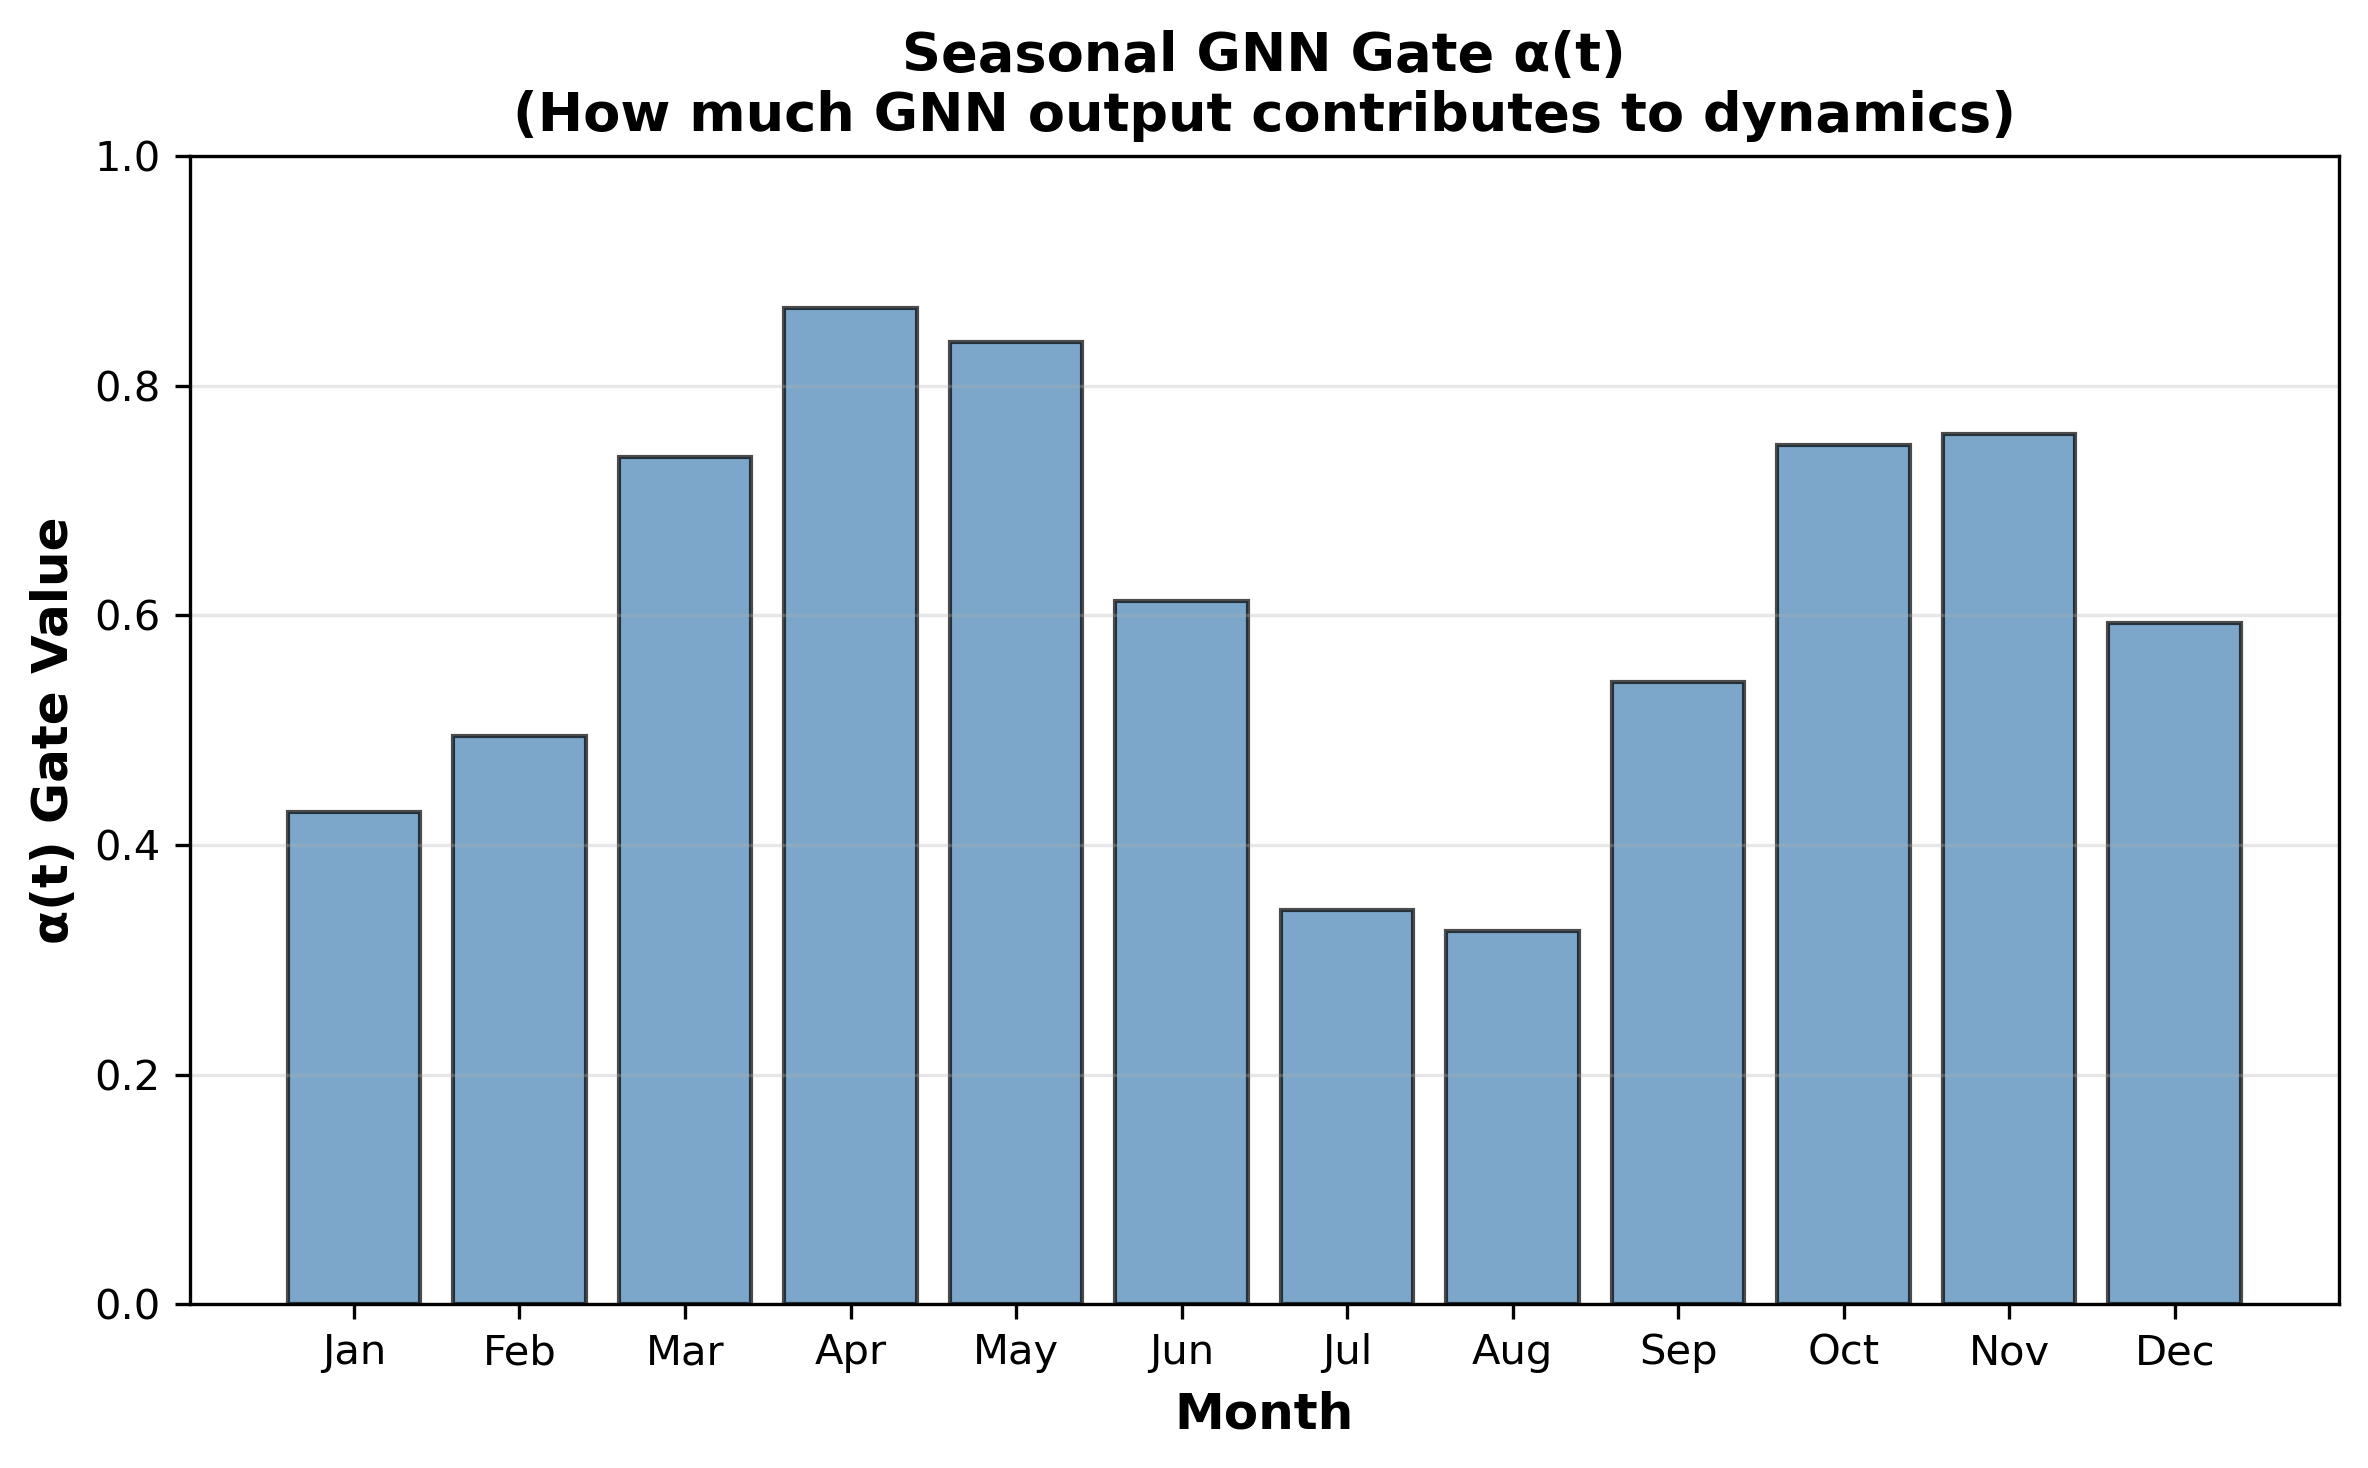
\includegraphics[width=\linewidth]{figures/gcn_seasonal_gate.png}
    \caption{The learned seasonal coupling $\alpha(t)$ for the NXRO-GNN model. Larger values indicate stronger impacts from the nonlinear terms.}
    \label{fig:seasonal_coupling}
\end{figure}







\section{Probabilistic Forecasting with Stochastic Dynamics}
\label{sec:stochastic}

Deterministic forecasts, while useful for point predictions, provide no quantification of uncertainty. Since weather and climate-based forecasts can impact decision-making in applications such as agriculture, water resource management, and disaster preparedness,  probabilistic forecasts that characterize the range of possible outcomes are essential~\cite{gneiting2014probabilistic}. For ENSO specifically, stochastic forcing from atmospheric noise and wind plays a fundamental role in the irregularity of the oscillation~\cite{kleeman2008stochastic}. In this section, we extend the NXRO-Residual framework to generate ensemble forecasts and develop a principled approach to calibrating the stochastic forcing that drives ensemble spread.

\paragraph{Probabilistic Evaluation Metrics: }Evaluating probabilistic forecasts requires metrics that assess both the accuracy of the ensemble mean and the reliability of the uncertainty estimates. We employ the Continuous Ranked Probability Score (CRPS)~\cite{hersbach2000}, a proper scoring rule~\cite{gneiting2007} that generalizes mean absolute error to probabilistic forecasts. The CRPS equals zero for a perfect forecast and increases as the forecast distribution deviates from the observation either in location or spread.  Forecasts that are overconfident (too narrow) are penalized when observations fall in the tails, while forecasts that are underconfident (too wide) are penalized for lacking sharpness. The score is expressed in the same units as the forecast variable (degrees Celsius for temperature), facilitating interpretation. For ensemble forecasts with $M$ members $\{x_1, \ldots, x_M\}$, we employ the fair CRPS estimator that corrects for finite ensemble size:
\begin{equation}
    \text{CRPS} = \frac{1}{M}\sum_{m=1}^{M} |x_m - y| - \frac{1}{2M^2}\sum_{m=1}^{M}\sum_{n=1}^{M} |x_m - x_n|
    \label{eq:crps_fair}
\end{equation}

\paragraph{Stochastic Model Formulation: }A key question in probabilistic forecasting is how to represent the stochastic component that drives ensemble spread. Traditional approaches in numerical weather prediction use stochastically perturbed parameterization tendencies (SPPT)~\cite{buizza1999stochastic}, which multiply physical tendencies by random numbers to represent model uncertainty. For reduced-complexity climate models like XRO~\cite{zhao2024xro}, the standard approach models stochastic forcing as  AR(1) process with seasonally-varying amplitude, fitted post-hoc from model residuals. We adopt this general framework but introduce a likelihood-based optimization procedure that improves upon post-hoc fitting.

In particular, we generate ensemble forecasts by adding stochastic forcing to the deterministic NXRO dynamics. The discrete-time stochastic model takes the form:
\begin{equation}
    \bX_{t+1} = \bX_t + \Delta t \cdot f_\theta(\bX_t, t) + \epsilon_t
    \label{eq:stochastic_model}
\end{equation}
where $f_\theta$ is the deterministic drift (either the full NXRO model or the XRO baseline), $\Delta t = 1/12$ years is the monthly time step, and $\epsilon_t$ is a stochastic perturbation. The perturbation follows a seasonal AR(1) process that captures the temporal correlation and seasonal amplitude modulation observed in forecast residuals:
\begin{equation}
    \epsilon_{j,t} = a_{1,j} \cdot \epsilon_{j,t-1} + \eta_{j,t}, \quad \eta_{j,t} \sim \mathcal{N}(0, (1 - a_{1,j}^2) \cdot \sigma_j(m)^2 \cdot \Delta t^2)
    \label{eq:ar1_noise}
\end{equation}
Here $a_{1,j} \in [0, 1)$ is the AR(1) persistence coefficient for variable $j$, controlling how quickly perturbations decay, and $\sigma_j(m)$ is the noise standard deviation for calendar month $m \in \{1, \ldots, 12\}$, allowing the noise amplitude to vary seasonally. The factor $(1 - a_{1,j}^2)$ ensures that the marginal variance of $\epsilon_{j,t}$ equals $\sigma_j(m)^2 \cdot \Delta t^2$ at stationarity.

% This noise model has $n + 12n$ parameters per model: one persistence coefficient per variable and twelve seasonal standard deviations per variable. The challenge is estimating these parameters in a way that produces well-calibrated ensembles.

\paragraph{Noise Parameter Estimation}

The quality of probabilistic forecasts depends critically on how noise parameters are estimated. Poor calibration---ensembles that are too narrow or too wide---undermines the utility of uncertainty estimates for decision-making~\cite{vannitsem2021statistical}. The XRO model~\cite{zhao2024xro} estimates noise parameters post-hoc by fitting AR(1) models to one-step prediction residuals, an approach that is computationally simple but does not optimize for multi-step forecast calibration. 

\paragraph{Likelihood-Based Optimization:} While post-hoc fitting is computationally convenient, it treats the persistence ($a_1$) and amplitude ($\sigma$) parameters independently, ignoring their joint effect on the stationary distribution. This can lead to suboptimal calibration. Our proposed approach optimizes noise parameters via maximum likelihood while holding the dynamics model fixed. This two-stage procedure separates the learning of deterministic dynamics from stochastic parameters, similar in spirit to approaches in neural stochastic differential equations~\cite{li2020scalable,kidger2021neural}. Given residuals $\{r_t\}_{t=1}^{T}$ computed from the frozen model, the conditional log-likelihood under the AR(1) model is:
\begin{equation}
    \ell(a_1, \sigma) = \sum_{t=2}^{T} \log p(r_t | r_{t-1}; a_1, \sigma_{m_t})
\end{equation}
where $m_t$ denotes the calendar month at time $t$ and $p(r_t | r_{t-1}; a_1, \sigma)$ is the Gaussian density implied by Equation~\ref{eq:ar1_noise}. We maximize this likelihood using gradient ascent, initializing from the post-hoc estimates. Unlike post-hoc fitting, it accounts for the interaction between persistence and amplitude. We refer to this as \textit{Stage 2} fitting because it occurs after the dynamics model has been trained (Stage 1 being the deterministic fitting described in Section~\ref{sec:neural_ode}).

\subsection{Results}

\begin{figure*}[t]
  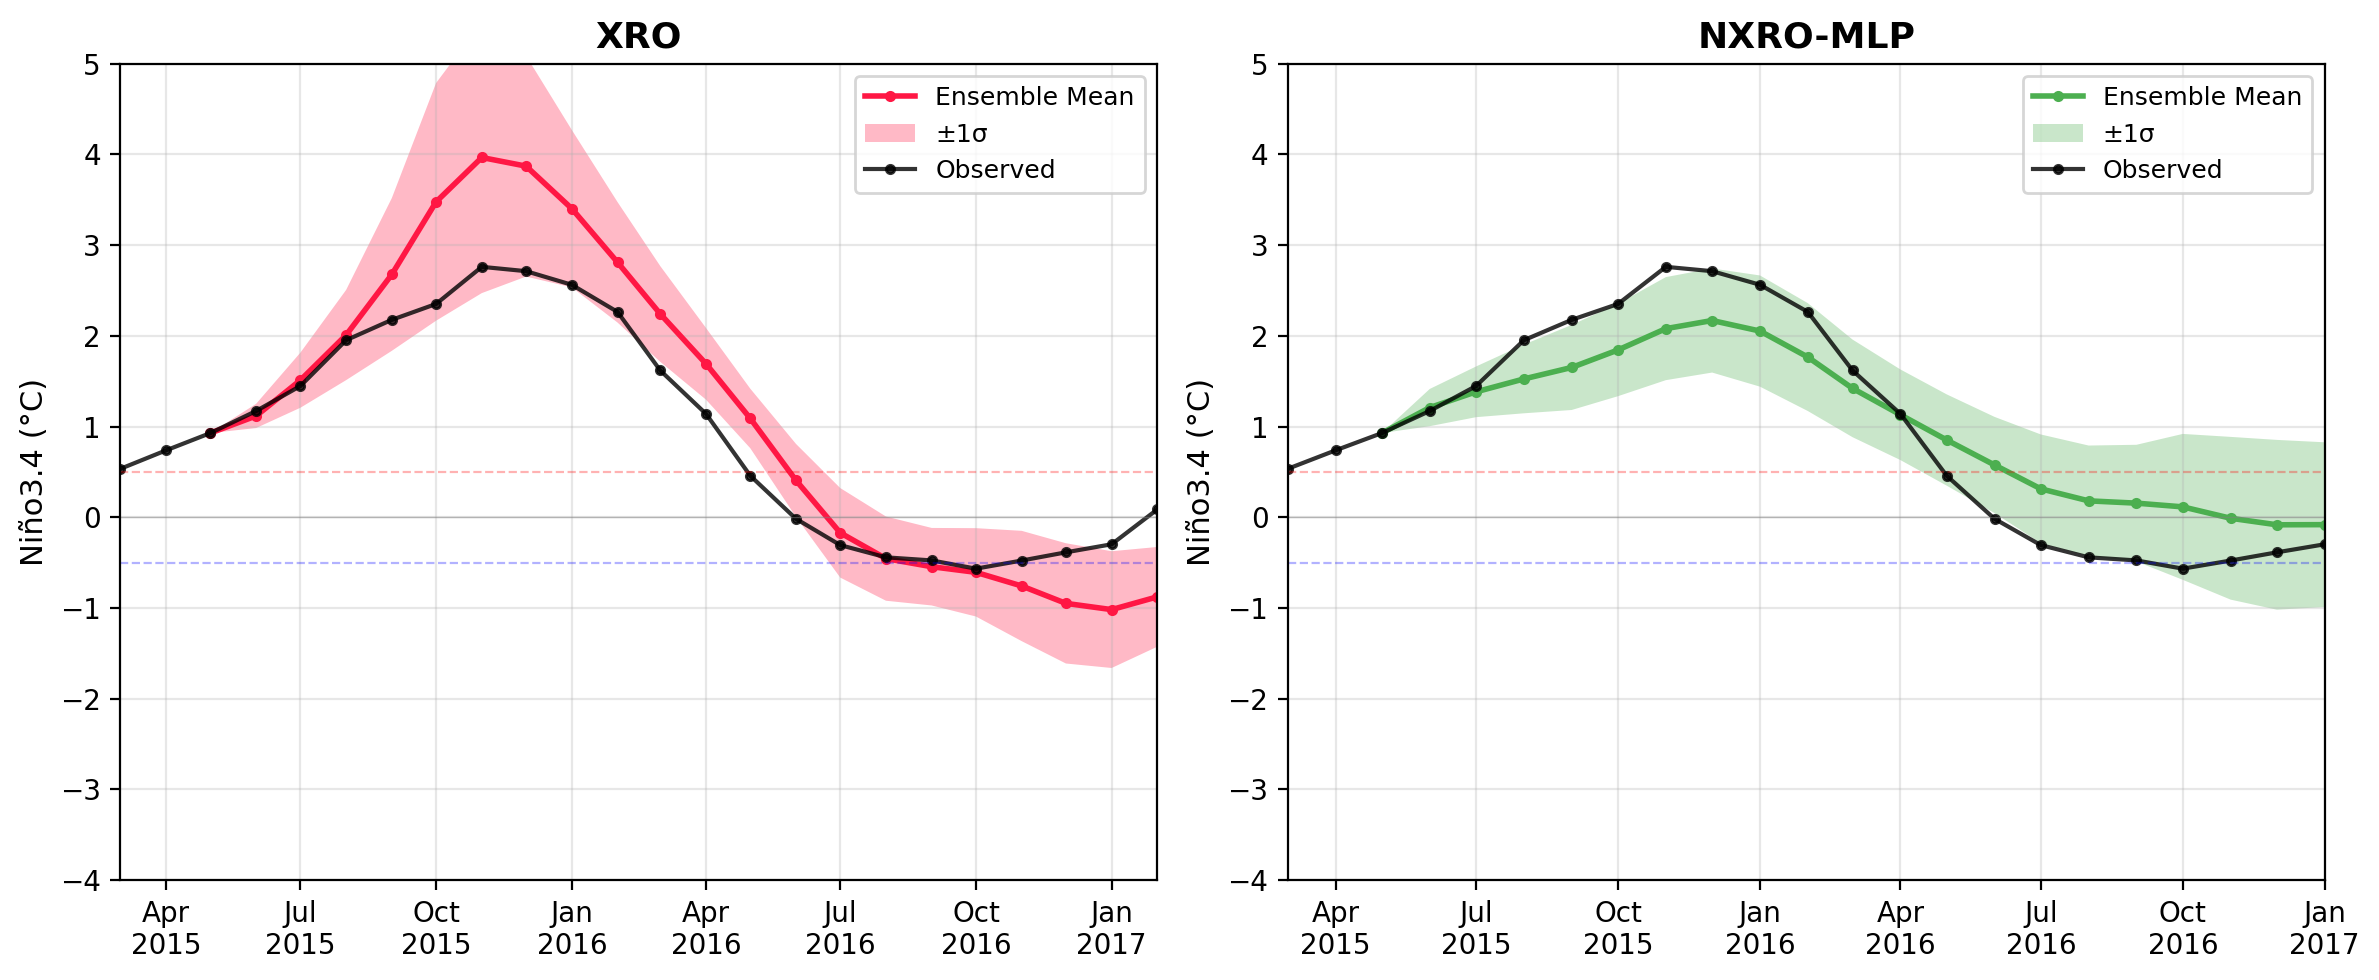
\includegraphics[width=\linewidth]{figures/elnino_2015_spring_xro_vs_mlp.png}
  \caption{Ensemble forecast comparison for the 2015 El Nino Spring development. Shaded regions show 10--90\% quantile ranges; solid lines show ensemble median; dots show observations. The NXRO-MLP model exhibits wider, better-calibrated spread.}
  \label{fig:forecast_samples_outsample}
\end{figure*}


Table ~\ref{tab:stochastic_outsample} presents the stochastic forecast performance for the out-of-sample evaluation. The results reveal striking differences between the noise estimation approaches. All NXRO variants with Stage 2 noise optimization outperform the XRO baseline, with up-to 13.0\% improvement in CRPS, achieved by the NXRO-GNN model, which is a meaningful advance for operational forecasting. In addition to CRPS, we also report Spread over RMSE, calculated as the ratio between standard deviation of ensemble forecasts and RMSE of the ensemble mean, averaged over all the lead times. The XRO baseline achieves a spread-to-RMSE ratio of only 0.527, indicating that its ensembles are overconfident. Stage 2 optimization increases this ratio to 0.625-0.654 across NXRO variants, moving closer to the ideal of 1.0. Better calibration means that users can more reliably interpret the ensemble spread as representing forecast uncertainty. %\YS{define spread to rmse. use the same term in Table 2. }

\begin{table}[h]
\setlength{\tabcolsep}{1pt}
\centering
\caption{Stochastic ensemble forecast performance for NXRO and XRO. Higher CRPS metrics means better calibration. }
\label{tab:stochastic_outsample}
\resizebox{\columnwidth}{!}{
\begin{tabular}{lcccc}
\toprule
\textbf{Model} & \textbf{CRPS} 
& \textbf{\shortstack{Ensemble\\RMSE}} 
& \textbf{\shortstack{Spread \\ over RMSE}} 
& \textbf{\shortstack{vs. \\ XRO}} \\
\midrule
NXRO-GNN & \textbf{0.488} & \textbf{0.899°C} & \textbf{0.654} & \textbf{$-$13.0\%} \\
NXRO-Attentive & 0.513 & 0.901°C & 0.634 & $-$8.6\% \\
NXRO-MLP & 0.548 & 0.963°C & 0.625 & $-$2.4\% \\
XRO & 0.561 & 0.970°C & 0.527 & --- \\
\bottomrule
\end{tabular}
}
\end{table}
\vspace{-9pt}
\subsection{Forecast Visualization}

Figure~\ref{fig:forecast_samples_outsample} illustrates an example of stochastic forecast with XRO and NXRO-MLP through ensemble plumes. The XRO ensemble (left panel) exhibits wide spreads that result in excessive uncertainty estimate, while missing observations. The NXRO-MLP ensemble (right panel) shows appropriately tighter spread that better represents forecast uncertainty while maintaining a more accurate ensemble mean, fitting the observations shape better and exhibiting better calibration. Additional stochastic forecast results can be found in Appendix B.

